\chapter{Fretha的设计和开发}

\section{引言}

\ifshowtext
在现代生物医学研究中,FRET双杂交分析作为一种关键技术,用于检测生物分子间的相互作用,为揭示生物过程的分子机制提供了重要手段。
然而,传统的 FRET 双杂交分析数据处理过程繁琐且效率低下,严重依赖人工操作,容易引入误差。
开发专门针对 FRET 双杂交分析数据处理的配套软件,能够实现数据的自动化采集、标准化处理以及高效的分析统计,对于提升研究效率和准确性具有重要意义。
本章节首先根据我们组自研的用于高通量药物筛选的 FRET 显微成像系统(FRETscopeII)的硬件参数和 FRET 数据处理及 FRET 双杂交分析数据处理功能进行深入的需求分析。基于此需求分析,对软件按照功能进行科学合理的模块划分和总体框架设计。
接着,详细介绍软件的开发技术选型以及每个模块的具体实现方式,旨在全面展示 Fretha 软件从设计构思到开发实现的全过程。
\fi

\section{需求分析和总体设计}

\subsection{需求分析}

\ifshowtext
% FRET多模态显微成像系统(FRETscopeII)的硬件和数据特点;
FRETscopeII是本课题组自研的适用于$3^3$-FRET、E-FRET、Pb-FRET等多种定量FRET分析方法的FRET多模态显微成像系统。该系统具备高分辨率成像、多通道同步采集等先进特性,能够获取高质量的 FRET 三通道图像数据。

% FRET双杂交分析数据处理流程。
使用FRETscopeII对制备好的样本进行图像采集得到若干视野的FRET三通道图像后,通过FRET双杂交分析方法定量计算细胞中的生物大分子结合作用的FRET饱和效率、化学计量比、相对亲和力等信息。FRET双杂交分析的数据处理需要如下步骤:首先需要对FRET数据进行数据完整性校验,确保每个视野下存在完整的三通道图像和文件完整可读,然后对每个视野进行荧光信号提取,通过在图像上绘制ROI并计算其灰度均值作为FRET分析计算重要的荧光信号;根据E-FRET和$3^3$-FRET方法将上述荧光信号代入对应的计算公式求取$E_A$、$E_D$、$R_C$等FRET数据;对这些数据进一步依据物理含义或者数据分析进行异常值去除等数据预处理;最后是通过优化算法拟合Langmiur模型或者线性模型计算相关的参数。具体流程如图 \ref{fig:tha_data_process} 所示。

\begin{figure}[hbtp]
    \centering
    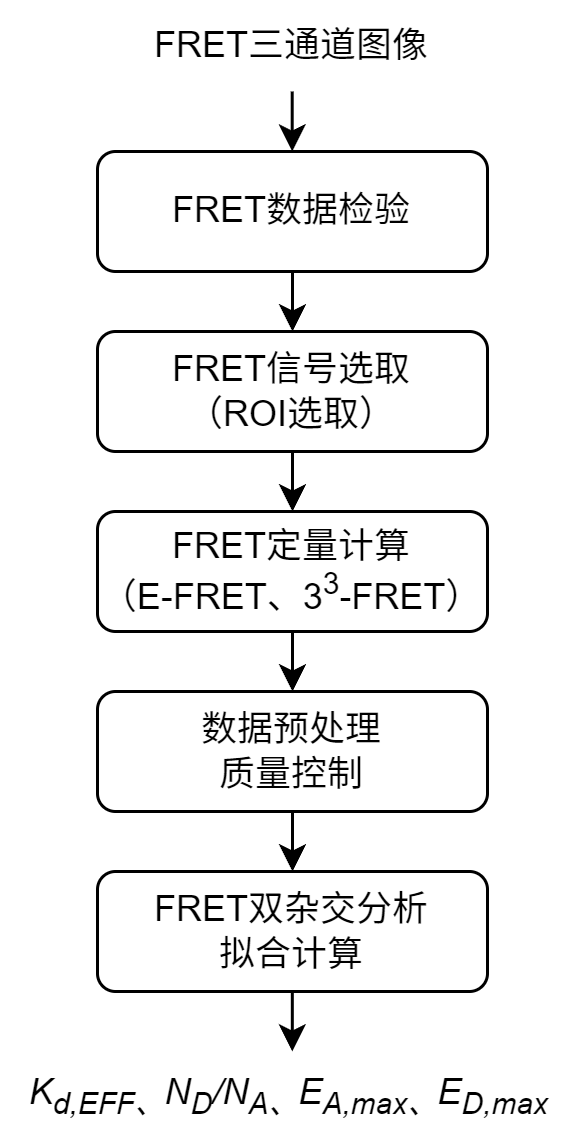
\includegraphics[width=0.4\linewidth]{../figures/2/2_FRET双杂交分析数据处理流程.png}
    \caption{FRET双杂交分析数据处理流程}
    \label{fig:tha_data_process}
\end{figure}

\fi

\subsection{模块划分}

结合 FRET 双杂交分析的数据处理流程与功能逻辑,Fretha 软件主要划分为以下核心模块:

\begin{enumerate}
  \item \textbf{成像参数设置模块:}负责设置 FRET 成像过程中的关键参数,确保成像数据的准确性和一致性。
  该模块允许用户输入和保存成像参数,如曝光时间、光学参数等,并提供参数校验功能,确保输入的参数在合理范围内,避免因参数设置错误导致的数据分析问题。
  成像参数一般比较稳定,通常2到3个月才需要重新测量,因此需要持久化到本地,以供多次处理数据时使用。
  \item \textbf{数据完备性检验模块:}对输入数据进行严格的完整性和合法性检验,避免异常数据导致的分析错误。
  该模块会检查每个视野的三通道图像文件是否完整,并对文件格式和内容进行验证,确保数据的可靠性。
  通过数据完备性检验,可以避免异常数据导致的分析错误,提高数据处理的准确性。
  \item \textbf{FRET 图像处理模块:}支持手动图像处理和 ROI 选取,满足用户对数据的精细化处理需求。
  用户可以在图像上手动圈选感兴趣区域(ROI),并进行图像增强、滤波等处理操作。
  该模块提供多种图像处理工具,帮助用户提高图像质量和分析精度。
  手动选取感兴趣区域ROI是一个基础且关键的操作,它能帮助分析人员聚焦于细胞中荧光质量较高的区域,进行更精确的数据处理与分析。
  \item \textbf{自动 ROI 圈点模块:}结合LURS(Luminance-Uniformity-based ROI Selection)算法实现自动 ROI 选取,显著提高数据处理效率。
  该模块利用机器学习算法自动识别和圈选图像中的感兴趣区域,减少人工操作,提高处理速度和一致性。
  自动圈点功能通过FRET双杂交求解器中封装的多线程服务,在不影响Fretha前台界面显示和操作的前提下,实现了一键式线程分离的自动数据处理。
  \item \textbf{结果可视化模块:}将分析结果以直观的图表形式展示,并提供数据保存功能,方便用户进一步分析和应用。
  该模块支持多种图表类型,如趋势线图、散点图等,用户可以根据需要选择合适的图表进行数据展示和分析。
  通过结果可视化,用户可以更直观地理解分析结果,比如分析FRET双杂交分析结果的相关性、拟合程度等,从而确保数据处理的准确性和可靠性。
  结果可视化模块还可以将分析结果保存为图片或数据文件,方便用户进行后续数据处理和报告撰写。
  
\end{enumerate}

\subsection{软件总体框架}

Fretha架构采用分层设计,由顶层向下依次分别为:表现层、业务层、数据访问层和数据层,如图\ref{fig:fretha_arch}所示。

\begin{figure}[hbtp]
    \centering
    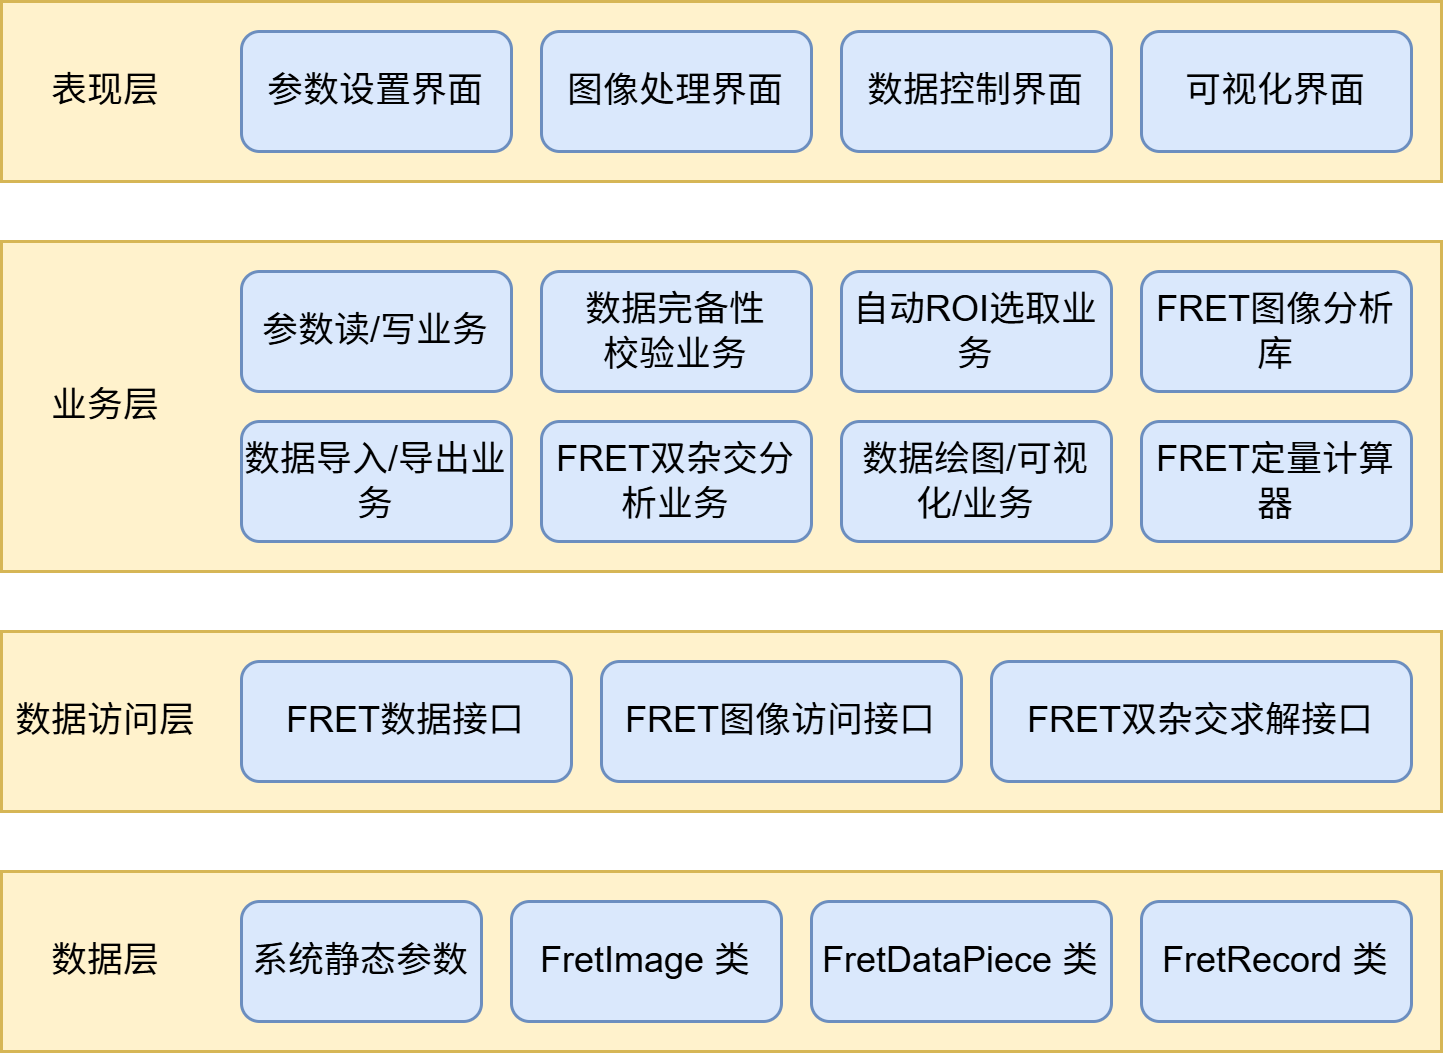
\includegraphics[width=1\linewidth]{../figures/2/2_Fretha软件架构图.png}
    \caption{Fretha软件总体架构}
    \label{fig:fretha_arch}
\end{figure}

表现层(Presentation Layer)处于整个架构的最外层,直接面向用户,是用户与系统进行交互的主要界面。
它负责接收用户输入的各种指令和数据,并以直观、友好的方式展示系统的处理结果。
Fretha的表现层主要包括参数设置界面、图像处理界面、ROI圈点界面、数据记录界面、可视化界面等,用户能够轻松地与系统进行交互,完成FRET双杂交分析的数据处理操作。

业务层(Business Logic Layer)是整个架构的核心逻辑处理部分,承担着对系统业务规则和流程的实现。
它接收来自表现层的请求,根据预设的业务逻辑对数据进行处理和转换。
Fretha的业务层封装了包括参数读/写业务、数据完备性检验业务、自动ROI选取业务、数据导入/导出业务、FRET双杂交分析业务、数据绘图/可视化业务等。
FRET定量计算器和FRET图像分析业务是业务层中进行FRET定量计算的业务,分别可以对FRET原始灰度数据和FRET图像数据进行定量FRET计算分析。Fretha中这两个业务为其他业务提供了关于FRET定量计算的数据处理能力,使得FRET定量分析及FRET双杂交分析数据处理过程中的科学计算逻辑进一步独立,减少了软件架构的冗余度,提高了编码以及程序运行的效率。

数据访问层(Data Access Layer)实现对数据的访问和操作,它将业务层与数据层进行隔离。
数据访问层提供了统一的数据访问接口,业务层通过调用这些接口来获取和存储数据,而无需关心数据的具体存储方式和位置。
通过设置数据访问层,能够使得在复杂的业务处理时避免对数据的直接操作和影响,从而提高了数据存储的安全性。
Fretha的数据访问包括FRET图像数据访问、FRET数值数据访问和FRET双杂交数据访问的接口。

最后是数据层(Data Layer),作为架构的最底层,数据层负责存储系统的所有数据。
Fretha数据层包括系统静态数据、FretImage类、FretDataPiece类和FretRecord类。
系统静态数据是在软件运行时的环境参数,只需要在指定步骤运行前提前设置好即可,如成像参数、文件目录等。
FretImage类、FretDataPiece类和FretRecord类用来表示数据处理时的各种动态数据。
在FRET双杂交分析数据处理中,一组FRET三通道图像中可以提取并计算出若干条FRET数据,由若干条FRET数据作为一个批次只能解析出一条FRET双杂交分析结果。
因此,在设计上三种数据实体类型存在关联关系,FretImage和FretDataPiece之间存在一对多的关系,FretDataPiece和FretRecord之间存在一对多关系,如图 \ref{fig:fretha_data_relations} 所示。

\begin{figure}[hbtp]
    \centering
    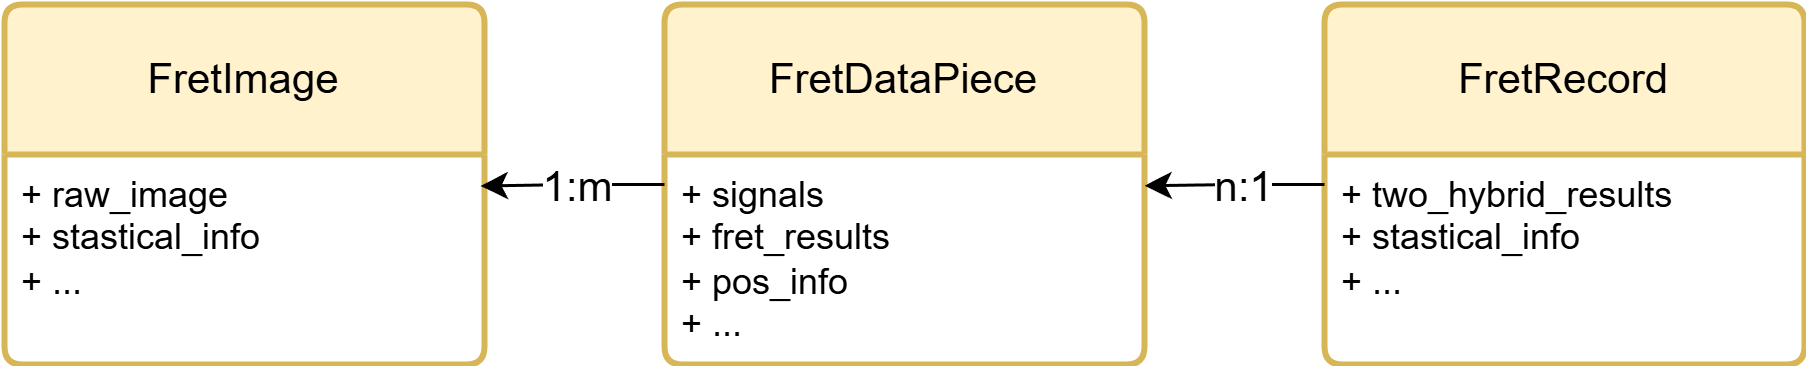
\includegraphics[width=1\linewidth]{../figures/2/2_Fretha数据层对应关系.png}
    \caption{Fretha数据层实体关联关系图}
    \label{fig:fretha_data_relations}
\end{figure}

\subsection{开发技术选型}
\ifshowtext
Qt 5.15.2是Qt官方发布的长期支持(LTS)版本,具有卓越的跨平台性能。该版本能够在Windows、Linux、macOS以及嵌入式系统等多种平台上稳定运行。
开发者只需对一套代码进行简单配置,即可实现不同平台的适配,这种特性大幅降低了软件开发与维护的成本。FRETscopeII的控制软件系统选择了Qt 5.15.2版本作为技术选型。
为了确保Fretha和FRETscopeII在开发过程中的一致性和可融合性,Fretha同样选用该版本作为软件开发的基础技术。
这一选择不仅有利于代码的共享、复用和维护,还能显著降低二次开发以及未来合并开发过程中的成本和风险。

在计算机视觉处理方面,Fretha选用了OpenCV(Open Source Computer Vision Library)。
OpenCV是一个开源的计算机视觉与机器学习软件库,具备强大的跨平台能力,可在Windows、Linux、macOS、Android、iOS等多种操作系统上运行。
其功能丰富多样,广泛涵盖了图像和视频处理的各个方面,例如图像的读取、滤波、边缘检测等。
在性能上,OpenCV经过SIMD指令集优化以及多线程并行计算等技术的优化,处理效率得到了显著提升,能够充分满足实时性的需求。
此外,OpenCV拥有一个活跃的社区,汇聚了大量的开发者。
社区中提供了丰富的算法、示例代码和实际案例,为开发者提供了有力的技术支持和学习借鉴的资源。
基于以上诸多优势,OpenCV完全契合本项目中计算机视觉任务的需求,因此被选定为本项目的重要技术工具。

在最优化计算方面,Fretha选择了C++库Dlib。
Dlib库集成了基于梯度的优化算法,并采用了自适应学习率机制,能够实现快速且稳定的收敛,有效降低了陷入局部最优解的概率。
该库还采用了牛顿法与拟牛顿法,在保证计算精度的同时兼顾了计算效率。
此外,Dlib在处理约束优化问题方面表现出色,例如可以运用内点法来解决资源分配中的约束难题,为研究工作提供了可靠的支持。  
\fi

\section{后台计算功能接口}

\subsection{FRET定量计算器}
FRET定量计算器(FretCalculator)用于处理E-FRET和$3^3$-FRET定量计算。FRET定量计算器定义了参数设置、数据加载、数据校正、数据计算和结果获取等计算步骤,每个步骤需要按照顺序执行,并且在执行时记录运行状态,在获取结果数据之前进行检查来保证数据安全。

\begin{figure}[hbtp]
  \centering
  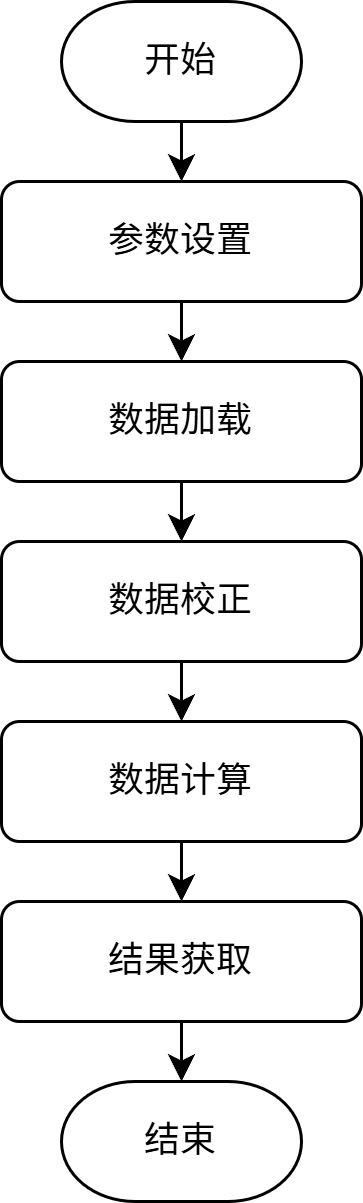
\includegraphics[width=0.25\linewidth]{../figures/2/2_FRET定量计算器流程.png}
  \caption{FretCalculator计算步骤}
  \label{fig:fretha_calculator}
\end{figure}

\subsection{FRET图像分析库}
FRET图像分析库(FretImageProcesser)封装了对FRET图像进行计算分析的计算器类,还静态方法的形式提供了图像处理算法的一系列接口。
首先按照FRET计算器的计算步骤对FRET图像数据进行处理,然后根据FRET图像数据的特点进行分析,完成逐像素的FRET计算,最后将计算结果保存到数据层中。
与FRET定量计算器不同,FRET图像分析时需要对每个像素点的荧光强度进行计算,因此需要对图像数据进行遍历处理。
FRET图像分析库采用OpenCV的Mat数据结构来存储图像数据。OpenCV提供的数据结构Mat是一个多维数组,可以方便地存储和处理图像数据,很适合存储逐像素的FRET图像数据。
FRET图像分析库的计算类FretImageProcesser的计算步骤和FRET定量计算器类似,如图 \ref{fig:fretha_calculator} 所示。

FRET图像分析库以静态方法的形式提供了FRET图像处理时涉及的一系列算法接口,包括图像预处理、图像分割、特征提取、图像增强等。所有的算法接口如表 \ref{tab:算法接口} 所示。
运用这些算法,FRET图像分析库支持了对16位原始数据的计算处理能力,以及可视化输出为伪彩图等功能。

\begin{table}[htb]
  \centering
  \caption{FRET图像处理库算法接口}
  \label{tab:算法接口}
    \begin{tabular*}{\textwidth}{p{0.3\textwidth}p{0.3\textwidth}p{0.4\textwidth}}
      \toprule[1.5pt]
      {\hei 接口} & {\hei 参数} & {\hei 说明} \\
      \hline

      morphologyClose & 
      \begin{tabular}[t]{@{}l@{}}
        Mat: 二值化图像 \\ 
        int: 迭代次数
      \end{tabular} & 
      形态学闭运算 \\

      morphologyOpen & 
      \begin{tabular}[t]{@{}l@{}}
        Mat: 二值化图像 \\ 
        int: 迭代次数
      \end{tabular} & 
      形态学开运算 \\
      
      medianFilter & 
      \begin{tabular}[t]{@{}l@{}}
        Mat: 单通道图像 \\ 
        int: 核大小
      \end{tabular} & 
      图像中值滤波 \\

      meanFilter & 
      \begin{tabular}[t]{@{}l@{}}
        Mat: 单通道图像 \\ 
        int: 核大小
      \end{tabular} & 
      图像均值滤波 \\
      
      gaussianFilter & 
      \begin{tabular}[t]{@{}l@{}}
        Mat: 单通道图像 \\ 
        int: 核大小 \\
        double: 高斯标准差
      \end{tabular} & 
      图像高斯平滑 \\
      
      getBackgroundValue & 
      Mat: 单通道图像 & 
      基于直方图的背景值估计 \\
      
      otsuThreshold & 
      \begin{tabular}[t]{@{}l@{}}
        Mat: 输入图像 \\ 
      \end{tabular} & 
      Otsu自动阈值分割 \\
      
      adaptiveThreshold & 
      \begin{tabular}[t]{@{}l@{}}
        Mat: 输入图像 \\ 
        int: 邻域大小(奇数) \\ 
        double: 阈值偏移量
      \end{tabular} & 
      自适应局部阈值分割 \\
      
      applyPseduoColor & 
      Mat: 单通道图像(8位) & 
      伪彩色映射(Jet颜色表) \\
      
      applyMask & 
      \begin{tabular}[t]{@{}l@{}}
        Mat: 输入图像 \\ 
        Mat: 掩膜(二值/同尺寸)
      \end{tabular} & 
      图像掩膜操作 \\
      
      minMaxNormalization & 
      Mat: 输入图像 & 
      全局线性归一化 \\
      
      mergeChannels & 
      \begin{tabular}[t]{@{}l@{}}
        Mat: R通道(8位) \\ 
        Mat: G通道(8位) \\ 
        Mat: B通道(8位)
      \end{tabular} & 
      多通道图像合并 \\
      \bottomrule[1.5pt]
    \end{tabular*}
\end{table}


\subsection{FRET双杂交求解器}
FRET 双杂交求解器对采集到的 FRET 批数据 $E_D$、$E_A$、$R_C$、$A_{est}$ 和 $D_{est}$ 进行最优化计算,以获取使预测结果与测量结果之间误差最小的$E_{A,max}$、$E_{D,max}$、$N_D / N_A$、$K_{d,EFF}$等参数。求解器从数据模型 FretRecord 中获取批量数据作为数据集,然后分别按照 DC - FRET 方法或 L - FRET 方法进行 FRET 双杂交分析求解。具体算法如下:
\begin{enumerate}
  \item \textbf{DC-FRET线性拟合算法的封装}。根据公式\ref{eq:ea_appro}和\ref{eq:ed_appro},DC-FRET拟合斜率时截距项为0。以参数$E_{A,max}$的拟合过程为例,其线性方程形式为
  \begin{equation}
      E_D = E_{A,max}\cdot R_C,
  \end{equation}
  其中,$E_D$是自变量,$R_C$是自变量,$E_{A,max}$是斜率。线性拟合的目标是找到合适的参数$E_{A,max}$,使得方程预测的$E_D$值与实际观测到的$E_D$值之间的误差尽可能小。
  通常使用最小二乘法,其原理是最小化观测值与预测值之间的误差平方和,即
  \begin{equation}
      S=\sum^{n}_{i=1}(E_{D_i}-(E_{A,max}R_{C_i}))^2
  \end{equation}
  其中,$n$是数据点的数量,$R_{C_i}$和$E_{D_i}$分别是第i个数据点的自变量和因变量的值。
  为了找到$S$最小的$E_{A,max}$值,对$S$关于$E_{A,max}$求偏导,并令其等于0。
  首先,展开误差$S$:
  \begin{align}
       S=\sum_{i = 1}^{n}(E_{D_i}^{2}-2E_{A,max}R_{C_i}E_{D_i} + E_{A,max}^{2}R_{C_i}^{2}), \\
       \frac{\partial S}{\partial E_{A,max}}=\sum_{i = 1}^{n}(-2R_{C_i}E_{D_i} + 2E_{A,max}R_{C_i}^{2}),
  \end{align}
  令 \(\frac{\partial S}{\partial E_{A,max}}=0\):
  \begin{align}
       \sum_{i = 1}^{n}(-2R_{C_i}E_{D_i} + 2E_{A,max}R_{C_i}^{2}) = 0, \\
      -2\sum_{i = 1}^{n}R_{C_i}E_{D_i}+2E_{A,max}\sum_{i = 1}^{n}R_{C_i}^{2}=0,
  \end{align}
  最后求解$E_{A,max}$:
  \begin{equation}
         E_{A,max}=\frac{\sum_{i = 1}^{n}R_{C_i}E_{D_i}}{\sum_{i = 1}^{n}R_{C_i}^{2}}. \label{eq:linear_fit_quick}
  \end{equation}
  公式 \ref{eq:linear_fit_quick} 给出了线性拟合求解的解析公式,可用于直接计算斜率$E_{A,max}$和$E_{D,max}$,从而避免了基于迭代的线性拟合求解算法的消耗。

  \item \textbf{L-FRET Langmiur模型拟合算法的封装。}Langmiur模型具有模型的非线性和参数的复杂性,无法通过简单的解析式解析其求解公式。因此,我们引入dlib计算库进行复杂的参数拟合。

  数据类型ColumnVector类型用于存储双精度浮点数的列向量,在后续的计算和优化过程中承载参数向量和中间计算结果。
  ExperimentalData结构体用于存储来自实验采集到的数据集,该结构体包含四个std::vector<double>类型的成员变量:aest存储$A_{est}$相关的数据数组,dest存储$D_{est}$相关的数据数组,ea\_corr存储$E_A$预测值($E_{A,p}$)与测量值($E_{A,o}$)之间的误差,ed\_corr存储$E_D$预测值($E_{D,p}$)与测量值($E_{D,o}$)之间的误差。
  
  \begin{lstlisting}[language=C++]  
  // 定义列向量类型
  typedef dlib::matrix<double, 0, 1> ColumnVector;
  
  // 定义数据结构体,用于存储实验数据
  struct ExperimentalData {
      std::vector<double> aest;
      std::vector<double> dest;
      std::vector<double> ea_corr;
      std::vector<double> ed_corr;
  };
  \end{lstlisting}
  
  CalculateError函数用于计算单个数据点的误差。其数学定义为
  \begin{equation}
    \text{Error}(predicted, observed) = (predicted - observed)^2.
  \end{equation}
  通过计算预测值predicted和测量值observed的差值的平方,然后作为误差返回。
  此函数基于最小二乘法原理,将误差的平方作为衡量预测值与真实值偏离程度的指标,在后续的损失函数计算中被广泛应用。
  CalculateLoss函数负责计算模型在整个数据集上的整体损失。对于给定的ExperimentalData实例data和参数向量parameters。
  ObjectiveFunction函数是优化过程的目标函数。它接受参数向量parameters和指向ExperimentalData结构体的指针data\_ptr作为输入。函数内部将指针转换为ExperimentalData类型,然后调用CalculateLoss函数,以计算并返回基于当前参数和实验数据的损失值。该目标函数为优化算法提供了评估参数优劣的标准,优化算法通过不断调整参数来最小化该目标函数的值。
  
  \begin{lstlisting}[language=C++]
  
  // 计算整体损失
  double CalculateLoss(const ExperimentalData& data, const ColumnVector& parameters) {
      double total_error = 0.0;
      for (size_t i = 0; i < data.aest.size(); ++i) {
          double d_free = ((data.dest[i] - parameters(0) - data.aest[i] * parameters(1)) +
                           std::sqrt(std::pow(data.dest[i] - parameters(0) - data.aest[i] * parameters(1), 2) +
                                     4 * parameters(0) * data.dest[i])) / 2;
          double a_free = data.aest[i] - (data.dest[i] - d_free) / parameters(1);
          double ea_pred = parameters(2) * d_free / (d_free + parameters(0));
          double ed_pred = parameters(3) * a_free / (a_free + parameters(0) / parameters(1));
  
          total_error += CalculateError(data.ea_corr[i], ea_pred) + CalculateError(data.ed_corr[i], ed_pred);
      }
      return total_error;
  }
  
  // 目标函数,用于优化过程
  double ObjectiveFunction(const ColumnVector& parameters, void* data_ptr) {
      auto data = static_cast<ExperimentalData*>(data_ptr);
      return CalculateLoss(*data, parameters);
  }
  \end{lstlisting}
  
  {TwoHybridSolver} 函数接受四个 std::vector<double> 类型的参数,分别为 {aest\_data}、{dest\_data}、{ea\_corr\_data} 和 {ed\_corr\_data},这些参数代表实验数据,用于后续的参数拟合过程。函数返回一个 {ColumnVector} 类型的对象,该对象存储了经过拟合得到的参数。
  在函数内部,首先创建一个长度为 4 的 {ColumnVector} 对象 {starting\_point},并将其初始值分别设置为 1、1、0.5 和 0.5,作为参数拟合的起始点。
  创建一个 {ExperimentalData} 类型的对象 {data},将传入的四个实验数据向量存储在该结构体中,以便后续目标函数使用。
  使用 Lambda 表达式定义了一个目标函数包装器 {objective\_wrapper},该包装器接受一个 {ColumnVector} 类型的参数 {parameters},并调用 {ObjectiveFunction} 函数,将 {parameters} 和指向 {data} 的指针作为参数传递给 {ObjectiveFunction},返回其计算结果。
  使用 {dlib} 库中的 {find\_min\_using\_approximate\_derivatives} 函数进行优化。采用 {dlib::bfgs\_search\_strategy()} 作为搜索策略,该策略是一种拟牛顿法,用于在参数空间中寻找目标函数的最小值。使用 {dlib::objective\_delta\_stop\_strategy(1e - 7)} 作为停止策略,当目标函数的变化小于 {1e - 7} 时,停止优化过程。该函数以 {objective\_wrapper} 作为目标函数,{starting\_point} 作为初始参数,{-1} 作为最大迭代次数(表示不限制最大迭代次数),{0.01} 作为步长。
  最后,函数返回 {starting\_point},此时 {starting\_point} 存储的是经过优化后得到的拟合参数。
  
  \begin{lstlisting}[language=C++]
  // 双杂交求解器,进行参数拟合
  ColumnVector TwoHybridSolver(const std::vector<double>& aest_data,
                               const std::vector<double>& dest_data,
                               const std::vector<double>& ea_corr_data,
                               const std::vector<double>& ed_corr_data) {
      // 初始化起始点
      ColumnVector starting_point(4);
      starting_point = 1, 1, 0.5, 0.5;
  
      // 创建数据结构体
      ExperimentalData data = {aest_data, dest_data, ea_corr_data, ed_corr_data};
  
      // 定义目标函数包装器
      auto objective_wrapper = [&data](const ColumnVector& parameters) {
          return ObjectiveFunction(parameters, &data);
      };
  
      // 使用 dlib 进行优化
      dlib::find_min_using_approximate_derivatives(
          dlib::bfgs_search_strategy(),
          dlib::objective_delta_stop_strategy(1e-7),
          objective_wrapper,
          starting_point,
          -1,
          0.01);

      return starting_point;
  }
  \end{lstlisting}
\end{enumerate}

\subsection{Qt开发的接口设计}


\section{功能模块的实现}

\subsection{成像参数设置模块}
\ifshowtext
FRET定量分析中,在数据处理前需要设置好FRET定量计算过程中必须的参数,设置成像过程时的成像参数至关重要。

FRET成像参数在Fretha中以静态参数保存在软件内存中,是数据处理时的环境参数。其中,a、b、c、d、G、k和Y是FRET成像系统的光学参数,在前文中已介绍;ExpTimeAA、ExpTimeDD和ExpTimeDA是成像时三个探测通道的曝光时间,在FRET定量计算时需要根据曝光时间参数在各个通道归一化,然后才能进行计算。
Fretha中包括的所有成像参数如表 \ref{tab:fretha_param_list} 所示。

\begin{table}[htb]
  \centering
  \caption[FRET成像参数]{FRET成像参数}
  \label{tab:fretha_param_list}
    \begin{tabular*}{\textwidth}{cp{8cm}lc}
      \toprule[1.5pt]
      {\hei 参数} & {\hei 说明} & {\hei 意义范围} & {\hei 单位} \\
      \hline
      \text{a} & 供体激发时在DA通道的串扰系数 & $(0,1)$ & 无\\
      \text{b} & 所有的一切都在这里面。 & $(0,1)$ & 无\\
      \text{c} & 模板类文件。 & $(0,1)$ & 无\\
      \text{d} & 受体激发时在DA通道的串扰系数 & $(0,1)$ & 无\\
      \text{G} & 供体猝灭和受体荧光增强的比值         & $(0,+\infty)$ & 无\\
      \text{k} & 受体浓度和供体浓度相同时的荧光比值 & $(0,+\infty)$ & 无\\
      \text{Y} & 供受体在激发光条件下的消光系数之比,也记作$\varepsilon_{YFP}(\lambda)/\varepsilon_{CFP}(\lambda)$   & $(0,+\infty)$ & 无\\
      \text{ExpTimeDD} & DD通道下的成像曝光时间 & $(0,+\infty)$ & 毫秒(ms)\\
      \text{ExpTimeDA} & DA通道下的成像曝光时间 & $(0,+\infty)$ & 毫秒(ms)\\
      \text{ExpTimeAA} & AA通道下的成像曝光时间 & $(0,+\infty)$ & 毫秒(ms)\\
      \bottomrule[1.5pt]
    \end{tabular*}
\end{table}

成像参数设置模块在业务设计上遵循一定的原则。首先,设置时所有参数应一同更新,避免因参数不匹配导致的数据处理错误。其次,每个参数需要在其有意义的范围内,避免无意义的值。
因此,在点击“更新参数”按钮时,若无法从界面中的每个参数输入框都解析到合法的数字,那么本次更新参数就会失败。
这是因为FRET成像参数是一批参数,参数间存在依赖关系,如测量参数$G$、$k$、$Y$就依赖参数$a$、$b$、$c$、$d$,这是因为测定参数$G$、$k$、$Y$时需要计算敏化发射荧光$F_C$,根据公式 \ref{eq:fc} 所示,$F_C$的确定与$a$、$b$、$c$、$d$密切相关。
强制所有参数一同更新可以避免用户单独设置某一参数而导致参数之间不匹配等问题。

FRET成像参数一般比较稳定,一般2到3个月才需要重新测量,因此需要持久化到本地,以供多次处理数据时使用。
Fretha的本地参数文件保存为可执行程序同级目录下的“config.ini”中。在软件初始化阶段,会自动检测并应用本地配置文件中的参数。
用户可通过保存多套配置文件,在使用时替换目标配置文件,快速进行参数配置的切换。

参数设置的业务流程如图 \ref{fig:fretha_param_module_flow} 所示。

\begin{figure}[hbtp]
    \centering
    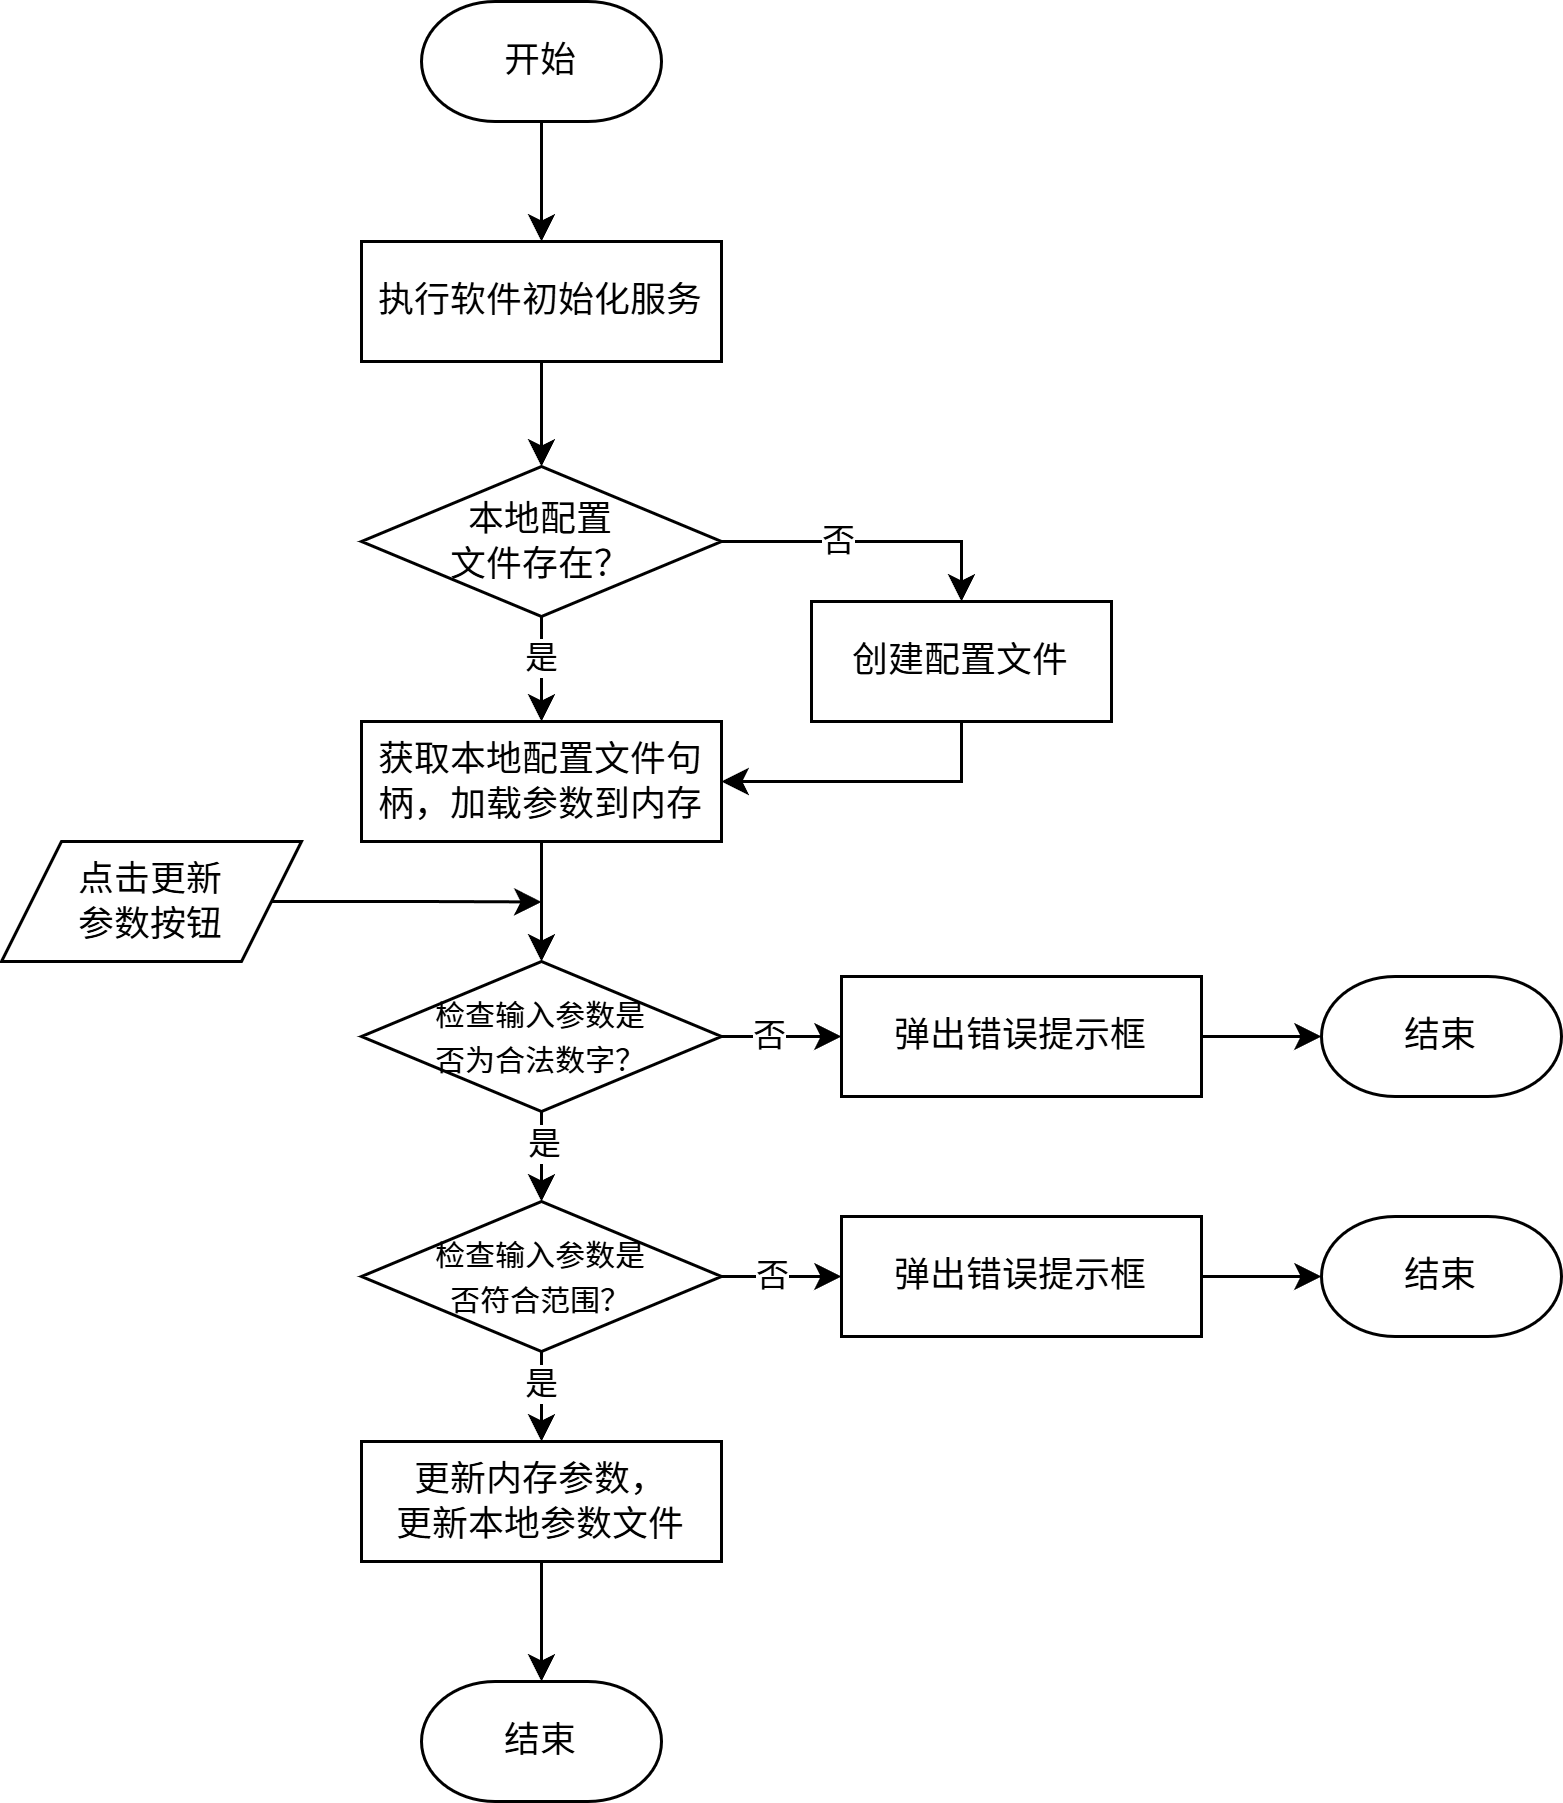
\includegraphics[height=1\linewidth]{../figures/2/2_成像参数设置模块业务流程.drawio.png}
    \caption{参数设置模块业务流程图}
    \label{fig:fretha_param_module_flow}
\end{figure}
\fi

\subsection{数据完备性检验模块}

FRET双杂交分析需要处理一批FRET图像文件,因此需要对输入数据的完备性进行检验识别。
该模块的作用有以下两个方面:一方面通过模式识别FRET合法数据,避免了异常输入导致的运行错误;
另一方面,在这一模块会将FRET批数据的视野子文件夹进行解析和类型识别,为后续数据处理提供对子文件夹的不同操作。

Fretha的数据识别检验模块匹配识别FRETscopeII的数据格式,从而保证数据处理能够正常开始。
FRETscopeII的数据结构由上层到下层依次为:(1)批数据根目录;(2)视野子目录;(3)图片数据和参数文件。
其结构如图 \ref{fig:fretscope_data_struct} 所示。

\begin{figure}[htbp]
    \centering
    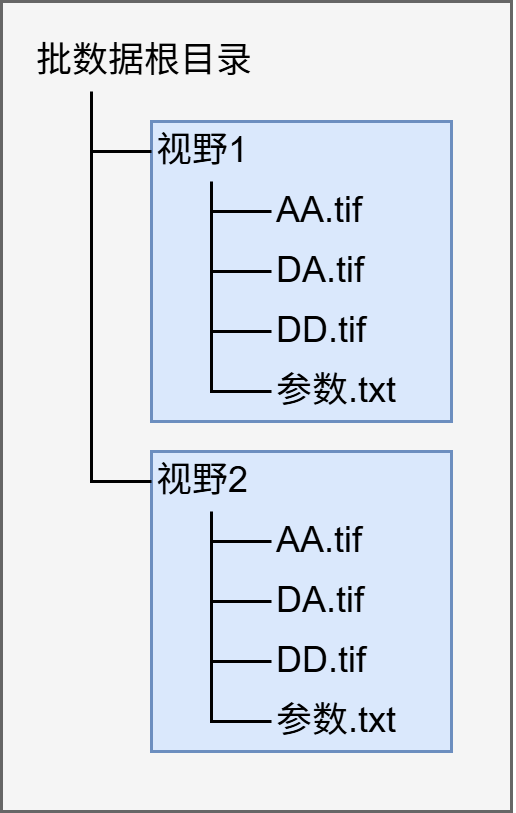
\includegraphics[height=0.5\linewidth]{../figures/2/2_FRETscopeII数据格式.drawio.png}
    \caption{FRETscopeII数据文件结构}
    \label{fig:fretscope_data_struct}
\end{figure}

数据完备性检验业务的流程如图 \ref{fig:fretha_data_check_flow} 所示。
其中,检查子文件夹类型是通过图 \ref{fig:fretscope_data_struct} 进行匹配的,当且仅当子文件夹中同时存在“DA.tif”、“DD.tif”和“AA.tif”图片文件时,当前子文件夹会被识别为FRET视野,并在视野表格模型中记录。
其他情况的子文件夹会被记作“Unknown”文件夹,在后续FRET图像处理或者自动处理中被跳过。

\begin{figure}[htbp]
    \centering
    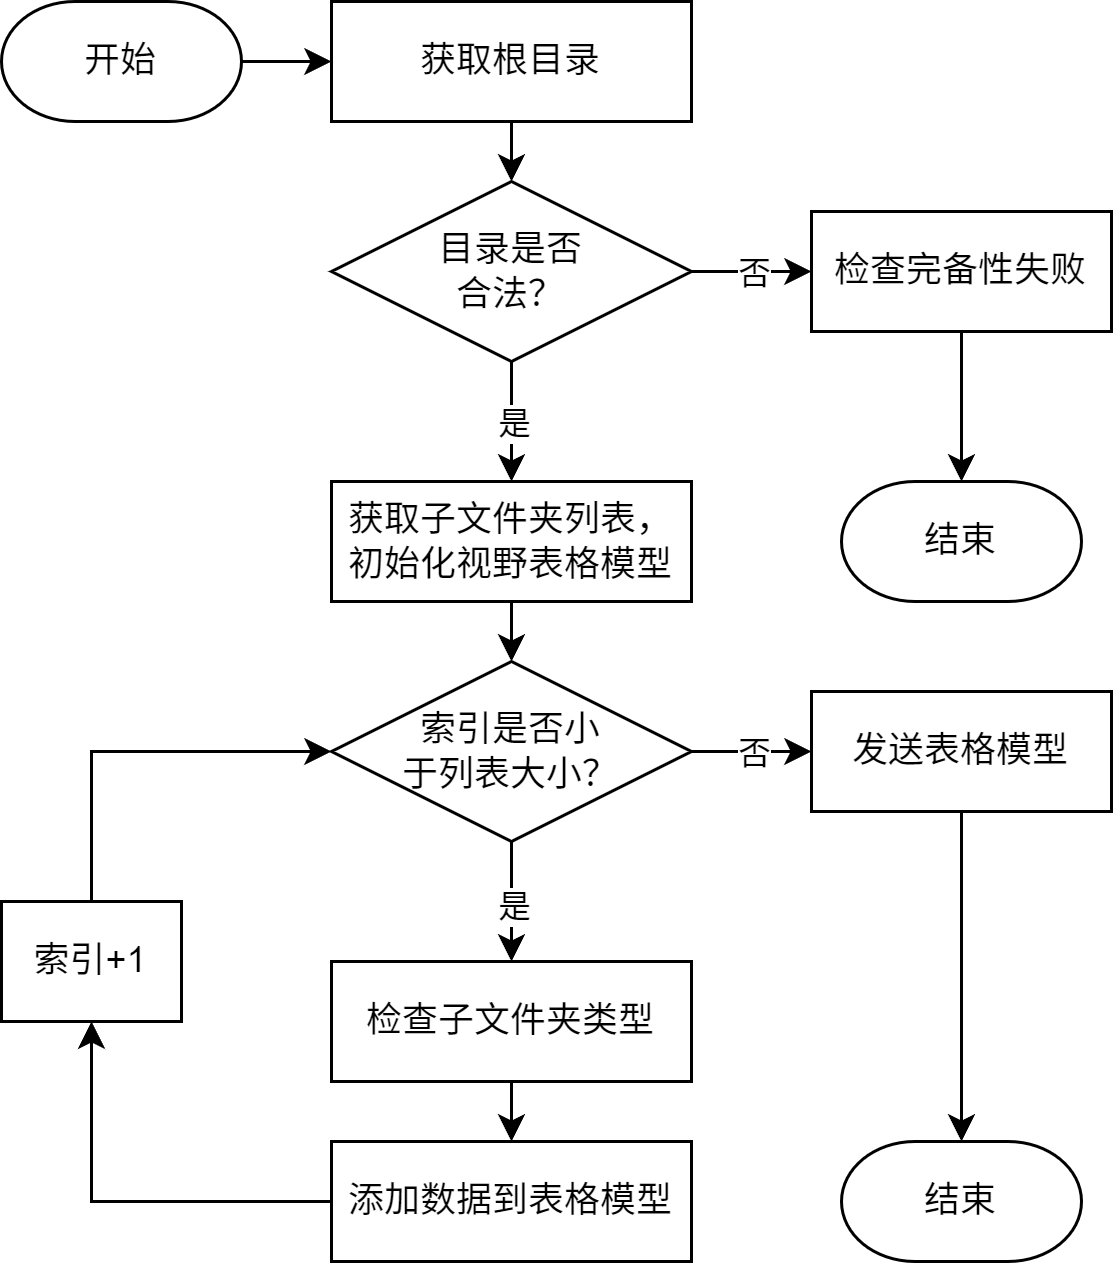
\includegraphics[width=0.6\linewidth]{../figures/2/2_数据完备性检验业务.drawio.png}
    \caption{Fretha数据完备性检验业务主流程图}
    \label{fig:fretha_data_check_flow}
\end{figure}

\subsection{FRET图像处理模块}

FRET图像处理模块是对FRET三通道图像进行ROI提取等图像处理分析的模块,包括手动ROI圈点和自动ROI圈点等。其界面如图 \ref{fig:fretha_imageprocess_ui} 所示:

\begin{figure}[htbp]
    \centering
    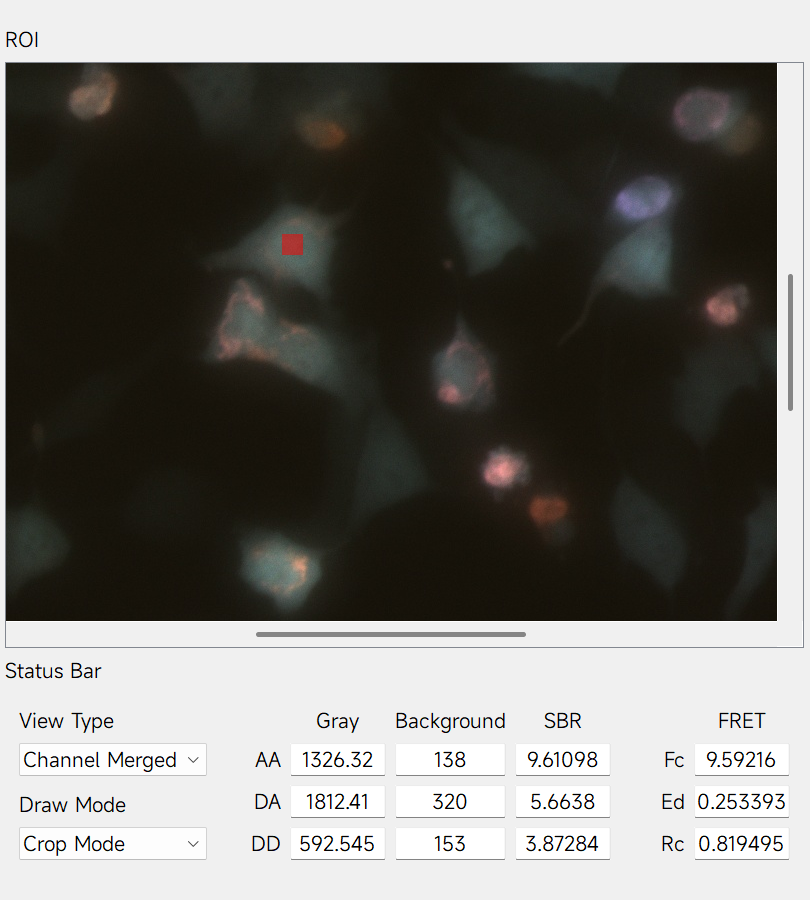
\includegraphics[width=0.75\linewidth]{../figures/2/2_图像处理模块界面.png}
    \caption{Fretha图像处理模块界面}
    \label{fig:fretha_imageprocess_ui}
\end{figure}

在FRET图像处理工作里,手动选取感兴趣区域ROI是一个基础且关键的操作,它能帮助分析人员聚焦于特定区域,进行更精确的数据处理与分析。
为达成图像处理过程中 ROI 的手动选取功能,Fretha 借助 Qt 框架提供的 QGraphicsView 类,开发了自定义的 FretGraphicsView 类。
QGraphicsView 是 Qt 用于可视化和交互处理二维图形场景的重要类,具备丰富的功能和良好的可扩展性,为 FretGraphicsView 的实现提供了有力支撑。

FretGraphicsView 类主要用于支持复杂的 ROI 编辑操作。
该类中新增了一个 ROI 成员,这一设计使 FretGraphicsView 具备了更完善的 ROI 管理能力。
它能够在视图中直观呈现 ROI 的大小和位置,方便用户确认所选区域。
同时,通过状态栏更新 ROI 内的数据,并为用户提供具有参考意义的FRET信息,有助于用户更深入地理解图像数据。

FretGraphicsView 通过自定义鼠标释放事件的信号,实现了与数据访问层的数据交互。
当用户完成 ROI 选取并释放鼠标时,FretGraphicsView 会将 ROI 的坐标和大小信息传递给数据访问层。
数据访问层依据当前视野索引,从数据模型中读取相应的三通道图像文件,并且从ROI信息提取FRET信号。
随后,这些数据会被输送至 FretCalculator 进行定量 FRET 计算。
计算完成后,原始灰度数据和 FRET 数据会更新到界面上,方便用户获取处理结果,为后续的数据分析工作提供依据。
这种基于 QGraphicsView 扩展的设计,有效提升了 ROI 选取的灵活性和准确性,实现了图像处理与数据计算的有机结合,为图像处理应用开发提供了一种可行的技术方案。 

Fretha的状态栏中提供了视图类型切换选项,在数据处理中可以辅助圈点,主要包括归一化增强图,和FRET伪彩图两类,支持的视图类型如表\ref{tab:fretha_viewtype_list}所示。
\begin{table}[htbp]
  \centering
  \caption[FRET图像视图类型]{FRET图像视图类型表}
  \label{tab:fretha_viewtype_list}
    \begin{tabularx}{\linewidth}{
    >{\centering\arraybackslash}X
    >{\centering\arraybackslash}X
    >{\centering\arraybackslash}X
    >{\centering\arraybackslash}X
    >{\centering\arraybackslash}X
    >{\centering\arraybackslash}X} % 修改第二列格式为p{6cm},可根据实际情况调整宽度
      \toprule[1.5pt]
      {\hei 信息} & {\hei 说明} \\
      \hline
      Channel Merged & 三通道归一合成图 \\
      DD Normalized & DD通道的归一化增强图 \\
      DA Normalized & DA通道的归一化增强图 \\
      AA Normalized & AA通道的归一化增强图 \\
      $R_C$ Pseudo & $R_C$逐像素数值伪彩图 \\
      $E_D$ Pseudo & $E_D$逐像素数值伪彩图 \\
      \bottomrule[1.5pt]
    \end{tabularx}
\end{table}
归一化增强图包括DD、DA、AA通道分别归一化的增强视图以及三通道归一化合成图。
FRET三通道原始图片由于测量系统的灰度量程为0至65535,在计算机显示时,灰度为65535的像素显示为纯白色,灰度为0的像素显示为纯黑。
然而,FRET信号往往达不到相机探测器量程的最大值,因此图片会显得灰暗,人眼识别图像中的细胞等问题。图像增强的计算公式如公式\ref{eq:normalize}所示。
\begin{equation}
\label{eq:normalize}
y = \frac{x - min_{old}}{max_{old}-min_{old}} \times (max_{new}-min_{new}) + min_{new}.
\end{equation}
其中,$x$是原图像中的像素值,$y$是经过归一化处理后的像素值,${min}_{old}$和${max}_{old}$分别是原图中像素灰度值的最小值和最大值,${min}_{new}$和${max}_{new}$分别是目标像素值中像素灰度值的最小值和最大值。
在图像显示时,我们将其设置为易于观察的0至255,因此公式\ref{eq:normalize}实际计算为:
\begin{equation}
\label{eq:normalize_255}
y = \frac{x - min_{old}}{max_{old}-min_{old}} \times 255
\end{equation}
除了视图辅助,Fretha状态栏能够清晰展示当前视野及ROI的状态信息,如当前视野的三通道背景灰度值、ROI信号的三通道信号背景比等,还可以显示使用当前ROI提供的扣除背景灰度值后的$I_{DD}$、$I_{DA}$和$I_{DD}$。
Fretha状态栏的所有显示内容如表\ref{tab:fret_statusbar_list}所示。
当对ROI调整完毕后,点击“添加数据”可以将ROI内的数据记录到软件右侧的表格中。
\begin{table}[htbp]
  \centering
  \caption[FRET圈点状态栏显示内容]{FRET圈点状态栏显示内容}
  \label{tab:fret_statusbar_list}
        \begin{tabularx}{\linewidth}{
    >{\centering\arraybackslash}X
    >{\centering\arraybackslash}X
    >{\centering\arraybackslash}X
    >{\centering\arraybackslash}X
    >{\centering\arraybackslash}X
    >{\centering\arraybackslash}X} % 修改第二列格式为p{6cm},可根据实际情况调整宽度
      \toprule[1.5pt]
      {\hei 信息} & {\hei 说明} \\
      \hline
      AA信号 & AA通道的ROI内灰度均值 \\
      DA信号 & DA通道的ROI内灰度均值 \\
      DD信号 & DD通道的ROI内灰度均值 \\
      AA背景 & AA通道的视野背景灰度值 \\
      DA背景 & DA通道的视野背景灰度值 \\
      DD背景 & DD通道的视野背景灰度值 \\
      \bottomrule[1.5pt]
    \end{tabularx}
\end{table}
点击左侧“自动圈点”按钮,可以使用LURS算法进行自动ROI圈点,并记录到右侧的数据记录表中。
自动圈点功能通过FRET双杂交求解器中封装的多线程服务,在不影响Fretha前台界面显示和操作的前提下,实现了一键式线程分离的自动数据处理。自动ROI圈点模块的业务流程及架构如图\ref{fig:fret_auto_roi_flow}所示。
架构层内的流程流转以实线表示,不同架构层之间的流程流转以虚线表示。
在实现自动圈点功能的流程转移中,发生在架构不同层之间的转移占更多数,而层内的流程转移相对较少,分层架构设计使得每个层内实现较好的封装,因此能够在实现复杂业务功能时,只需要专注于层和层之间的数据和流程切换即可。
LURS算法将会在第三章具体说明。
\begin{figure}[htbp]
    \centering
    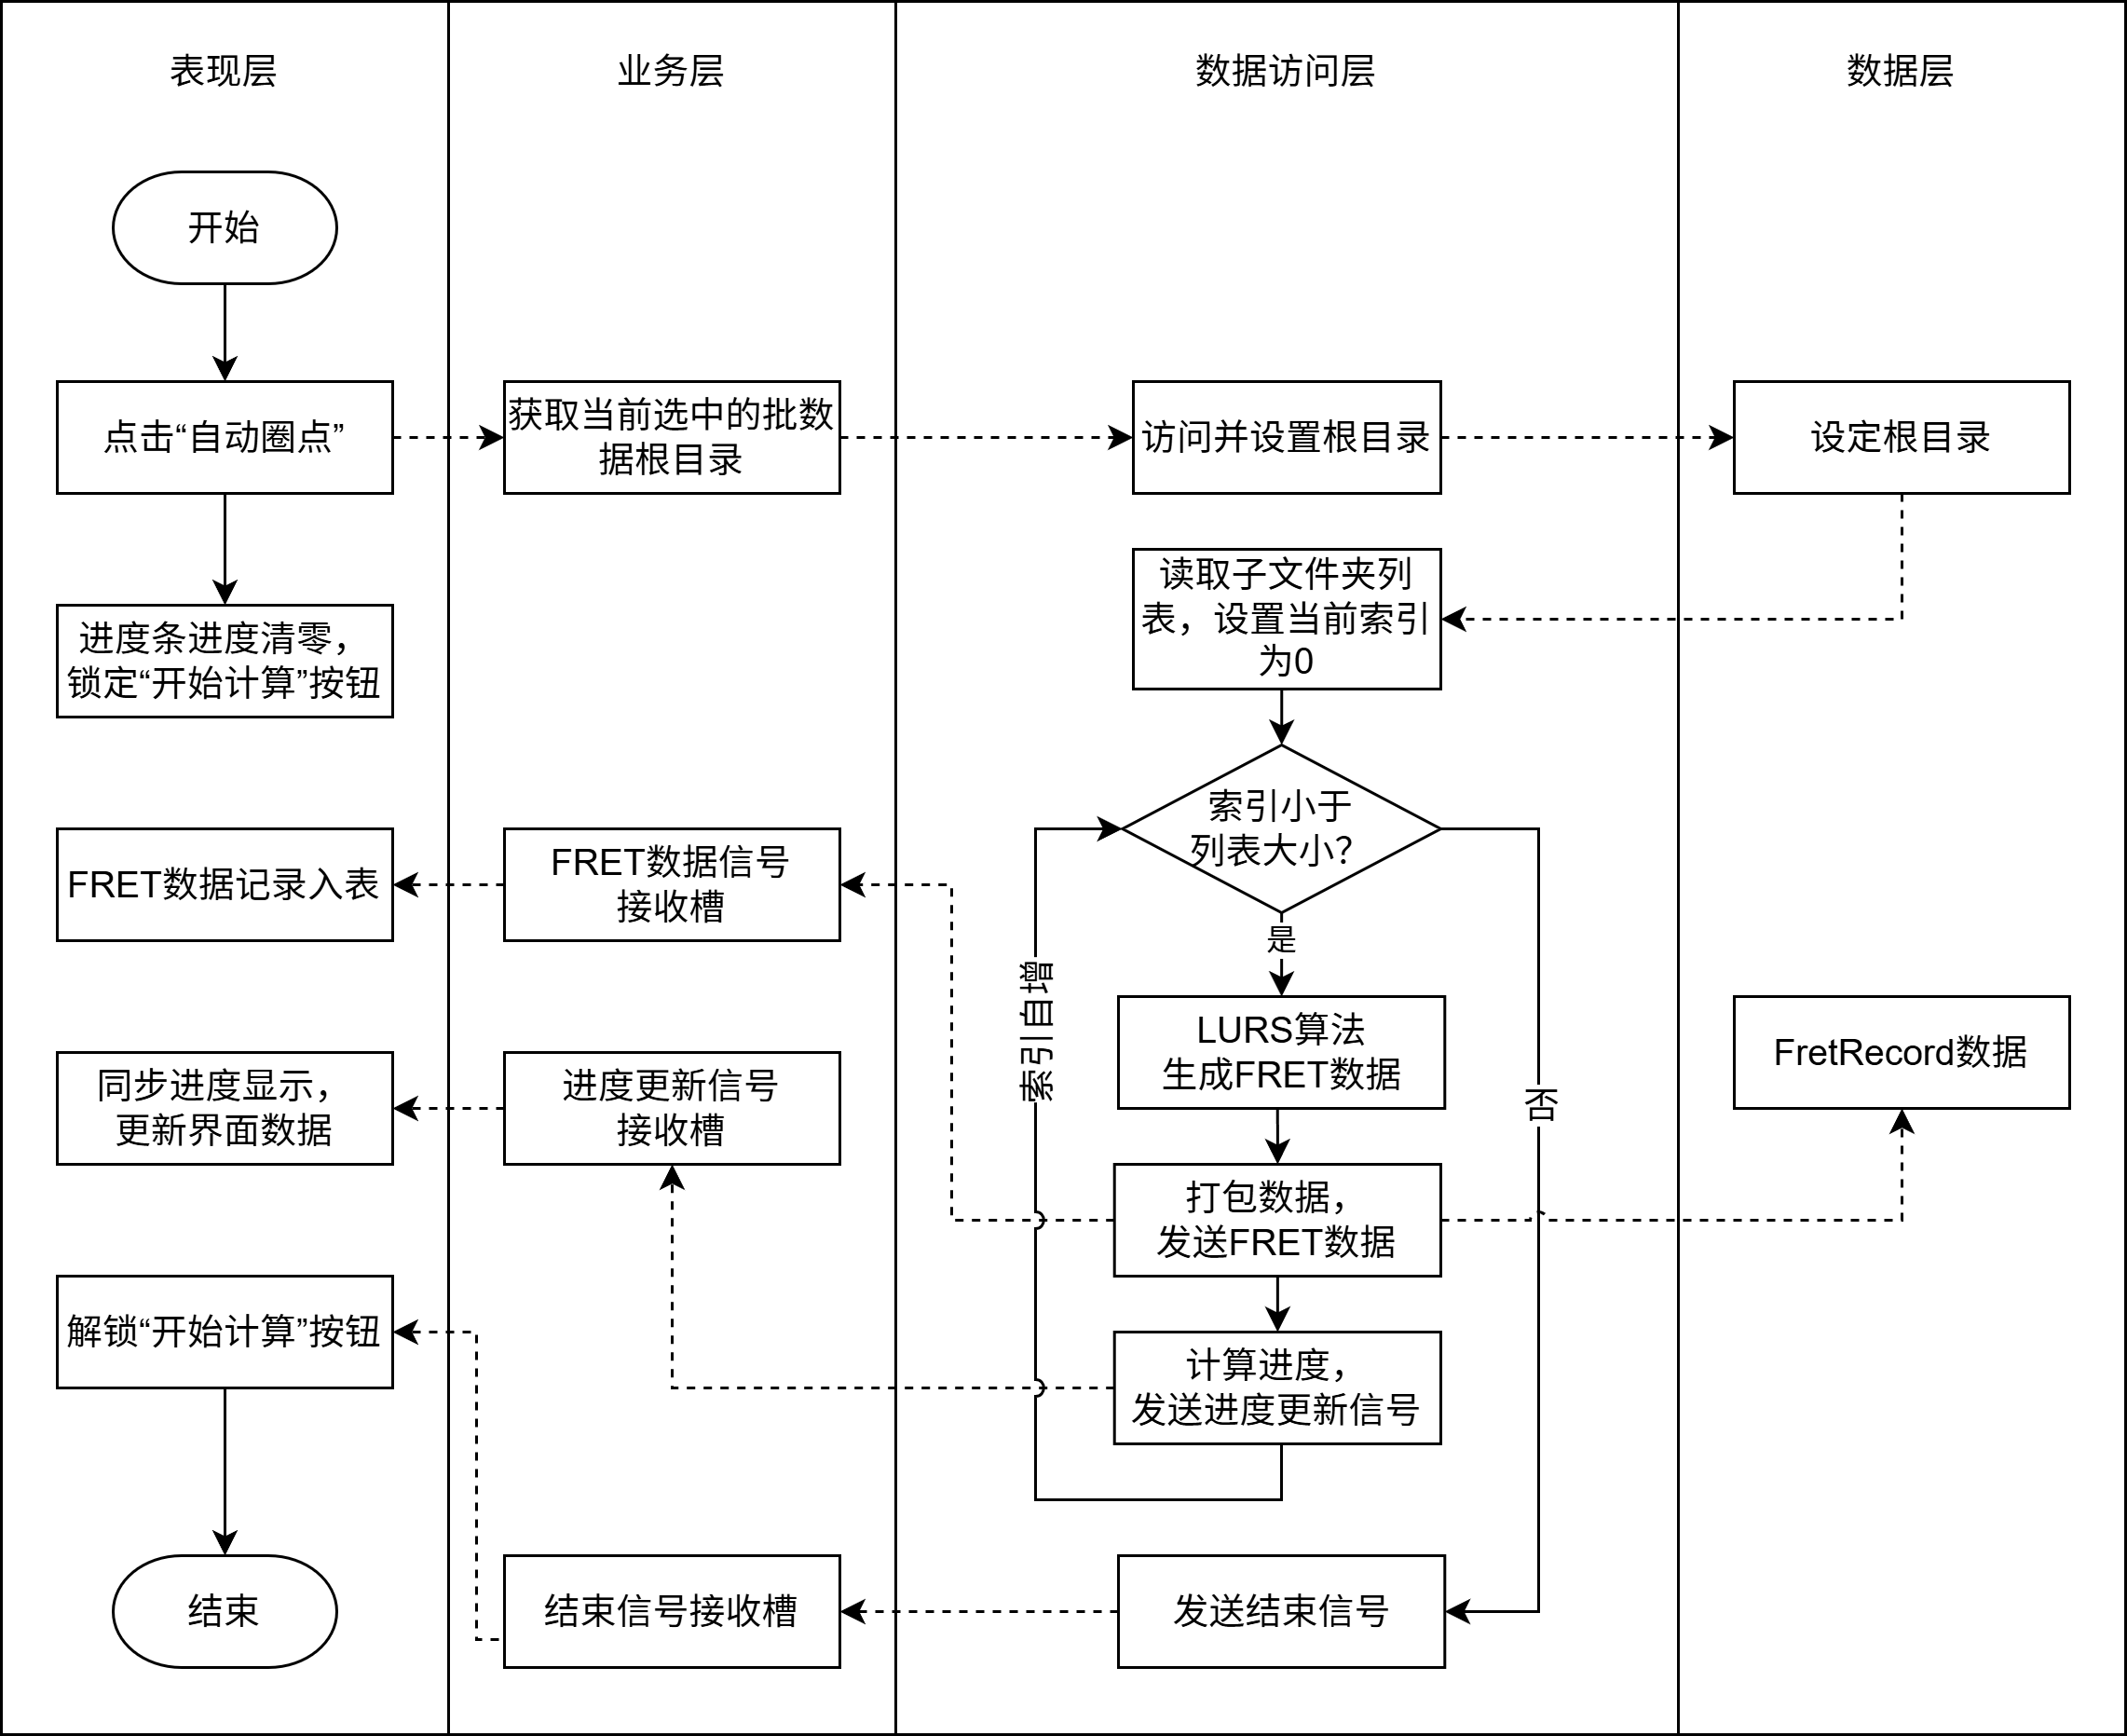
\includegraphics[width=1\linewidth]{../figures/2/2_自动ROI圈点模块业务流程.png}
    \caption{Fretha自动圈点模块流程}
    \label{fig:fret_auto_roi_flow}
\end{figure}

\subsection{数据控制模块}

数据控制模块支持对数据的实时操作,可以对于图像处理模块获得的数据,进行异常数据筛选、数据导入、数据导出、数据追踪、计算入口等数据控制功能。

在数据模型上,我们将一条数据类型FretDataPiece定义中包含数据如表 \ref{tab:数据项内容定义} 所示。
可以看出,FretDataPiece包含了一个ROI对应的所有原始信息,如ROI的位置、大小、信号强度、视野等;同时,还包含了计算后的$E_D$、$E_A$、$R_C$、$1/R_C$等中间参数,可以直接被用于后续的数据处理。

\begin{table}[hbtp]
  \centering
  \caption{FretDataPiece数据类型}
  \label{tab:数据项内容定义}
    \begin{tabularx}{\linewidth}{
    >{\centering\arraybackslash}X
    >{\centering\arraybackslash}X
    >{\centering\arraybackslash}X
    >{\centering\arraybackslash}X
    >{\centering\arraybackslash}X
    >{\centering\arraybackslash}X
    >{\centering\arraybackslash}X
    >{\centering\arraybackslash}X
    >{\centering\arraybackslash}X
    >{\centering\arraybackslash}X
    >{\centering\arraybackslash}X} 
      \toprule
      {\hei 信息} & {\hei 说明} \\
      \hline
      $I_{DD}$ & ROI在DD通道扣除背景后的信号强度 \\
      $I_{DA}$ & ROI在DA通道扣除背景后的信号强度 \\
      $I_{AA}$ & ROI在DD通道扣除背景后的信号强度 \\
      $E_D$ & 根据$I_{DD}$、$I_{DA}$、$I_{AA}$计算的$E_D$ \\
      $R_C$ & 根据$I_{DD}$、$I_{DA}$、$I_{AA}$计算的$R_C$ \\
      $E_A$ & 根据$I_{DD}$、$I_{DA}$、$I_{AA}$计算的$E_A$ \\
      $1/R_C$ & 根据$I_{DD}$、$I_{DA}$、$I_{AA}$计算的$1/R_C$ \\
      $x$ & ROI的横坐标 \\
      $y$ & ROI的纵坐标 \\
      $w$ & ROI的宽度 \\
      $h$ & ROI的高度 \\
      $view$ & ROI隶属的视野\\
      \bottomrule
    \end{tabularx}
\end{table}

异常数据筛选分为根据物理意义的筛选和统计离群检测两个部分。具体做法如下:
\begin{enumerate}
  \item 物理意义筛选。
  根据数据项的物理属性设定合理定义域。
  例如,$I_{DD}$应满足 $I_{DD} > 0$。对于数值型数据$X_i$,删除条件可表示为:
  \begin{equation}
    \text{删除条件} = 
      \begin{cases} 
        1, & \text{若} \ x_i \notin [L_i, U_i] \\
        0, & \text{其他情况}
      \end{cases}
  \end{equation}
  其中 $L_i$ 和 $U_i$ 为第 $i$ 个变量的定义域上下限,删除条件为1表示需要删去该数据。
  \item 统计离群检测。
  对通过物理筛选后的数据计算均值 $\mu$ 和标准差 $\sigma$,在FRET双杂交分析中主要对计算后的$E_D$和$E_A$进行筛选。构建离群点判定准则:
  \begin{equation}
      \text{离群阈值} = \mu \pm 3\sigma
  \end{equation}
  超出该范围的数据点视为离群点。具体步骤为:
  \begin{equation}
          \mu = \frac{1}{n}\sum_{i=1}^n x_i, \quad \sigma = \sqrt{\frac{1}{n-1}\sum_{i=1}^n (x_i - \mu)^2}
  \end{equation}
  

\end{enumerate}
首先根据各项数据的物理意义进行筛选,删除其中超出定义域的数据项。然后,删除超出数据中超过3倍标准差的离群数据。

数据导入和导出用于保存数据处理时的ROI信息。在一次FRET双杂交分析数据处理后,需要记录本次数据处理的处理数据,方便后续查看。导出的数据信息包括:

数据追踪是指在数据表格中点击某一条数据,软件会根据这条数据的位置和形状信息,在图像显示上显示该条数据对应的ROI位置,以方便识别数据中潜在的错误。实现这一功能,主要基于Qt提供的信号与槽机制。将数据中的数据模型被单机的事件与FretGraphicsView控件绑定后,FretGraphicView模型可以接收到来自所选数据的信息,并将当前活动的ROI按照所选数据的位置和形状重新绘制。

\subsection{结果可视化模块}
\ifshowtext
FRET双杂交分析的数据结果包括FRET数据进行双杂交计算的参数结果和拟合曲线图。
FRET双杂交分析数据拟合结果的参数是用户得到的核心结果,其中$n_D/n_A$、$K_{d,EFF}$等参数是生物学家最关心的生物大分子之间相互作用的参数。
FRET双杂交分析的拟合曲线图是将双杂交拟合曲线和实验采集到的散点同时绘制在一张图上,用于评估双杂交计算结果的拟合效果,以进一步判断FRET双杂交分析结果的可信度。

点击“保存结果”按钮后,上述数据结果和图片结果都将被保存,还将保存可在其他绘图软件上制图的原始数据,其中相比较圈点的数据来说,主要新增了$A_{free}$和$D_{free}$数据点,这部分信息的计算依赖于FRET双杂交分析的参数结果,在结果展示时才能确定。

结果可视化模块的界面主要包括三个部分:FRET双杂交分析算法选择;FRET双杂交分析图表结果;结果保存按钮。
\fi



\section{本章小结}

\ifshowtext
本章介绍了FRET双杂交分析数据处理软件(Fretha)的设计和开发。Fretha采用分层架构设计,被分为表示层、业务层、数据访问层和数据层,从设计上尽可能地进行解耦,减少了冗余设计。基于FRET双杂交分析数据处理的需求,Fretha在功能逻辑上划分为成像参数设置模块、数据校验模块、FRET图像处理模块、数据控制模块和结果可视化模块,然后通过分层架构完成了每个功能模块的开发。得益于分层架构设计和功能模块化设计,Fretha实现了各种复杂Fretha说明Fretha是一款拥有用户友好界面、简单易用、处理高效的科研数据处理软件。
\fi